\documentclass[11pt]{exam}

\usepackage{amsmath, amssymb, multicol}
\usepackage{graphicx}
\usepackage{textcomp}
\usepackage{chessboard}
\usepackage{tikz}

\def\d{\displaystyle}
\def\b{\mathbf}
\def\R{\mathbf{R}}
\def\Z{\mathbf{Z}}
\def\st{~:~}
\def\bar{\overline}
\def\inv{^{-1}}


\newcommand{\vtx}[2]{node[fill,circle,inner sep=0pt, minimum size=7pt,label=#1:#2]{}}
\newcommand{\va}[1]{\vtx{above}{#1}}
\newcommand{\vb}[1]{\vtx{below}{#1}}
\newcommand{\vr}[1]{\vtx{right}{#1}}
\newcommand{\vl}[1]{\vtx{left}{#1}}
\renewcommand{\v}{\vtx{above}{}}


%\pointname{pts}
\pointsinmargin
\marginpointname{pts}
\addpoints
\pagestyle{head}
%\printanswers

\firstpageheader{Math 228}{\bf Euler Paths}{Wednesday, November 15}


\begin{document}

%space for name
%\noindent {\large\bf Name:} \underline{\hspace{2.5in}}
%\vskip 1em

\noindent An \emph{Euler path} in a graph or multigraph is a path which uses every edge exactly once.  An \emph{Euler circuit} is an Euler path which starts and stops at the same vertex.  Your goal is to find a quick way to check whether a graph (or multigraph) has an Euler path or circuit.

\begin{questions}
\question Which of the graphs/multigraphs below have Euler paths?  Which have Euler circuits?


\begin{center}
 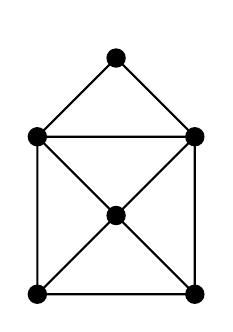
\begin{tikzpicture}
  \draw[thick] (-1,0) \v -- (1,0)\v -- (1,2) \v -- (-1, 2) \v -- (-1,0) -- (1,2) (-1,2) -- (1,0) (0,1) \v;
  \draw[thick] (-1,2) -- (0,3) \v -- (1,2);
\end{tikzpicture}
\hfill
 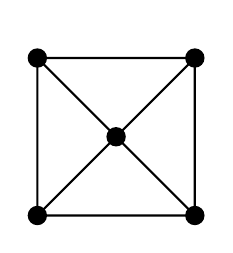
\begin{tikzpicture}
  \draw[thick] (-1,0) \v -- (1,0)\v -- (1,2) \v -- (-1, 2) \v -- (-1,0) -- (1,2) (-1,2) -- (1,0) (0,1) \v;
\end{tikzpicture}
\hfill
 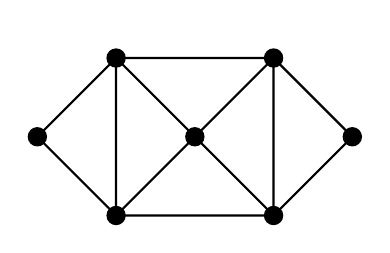
\begin{tikzpicture}
  \draw[thick] (-1,0) \v -- (1,0)\v -- (1,2) \v -- (-1, 2) \v -- (-1,0) -- (1,2) (-1,2) -- (1,0) (0,1) \v;
  \draw[thick] (-1,0) -- (-2,1) \v -- (-1,2) (1,2) -- (2,1) \v -- (1,0);
\end{tikzpicture}
\hfill
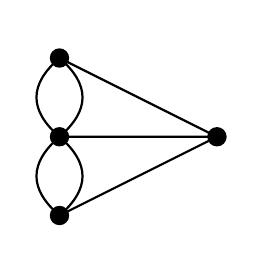
\begin{tikzpicture}[yscale=.5]
 \draw[thick] (-1,-2) \v to [out=120, in=240] (-1,0) \v to [out=120, in=240] (-1,2) \v to [out=300, in=60] (-1,0) to [out=300, in=60] (-1,-2);
  \draw[thick] (1,0) \v -- (-1,2) (-1,0) -- (1,0) -- (-1,-2);
  \end{tikzpicture}

\end{center}

\begin{solution}
The first graph has an Euler path but not a circuit.  The second graph doesn't have an Euler path or circuit. The third has an Euler circuit (which is a special type of Euler path).  The last graph (Bridges of K\"onigsberg) does not have an Euler path or circuit.
\end{solution}


\vfill
\question List the degrees of each vertex on the graphs above.  Notice anything?

\begin{solution}
The degree of a vertex is the number of edges incident (attached) to it.  The first graph has two vertices with degree 3, and the rest have degree 4 or 2.  The second graph has one vertex with degree 4 and four with degree 3.  The third graph has two vertices with degree 2 and the rest have degree 4.  The last graph has one vertex with degree 5 and the others have degree 3.  Notice that the graphs which do not have Euler paths have lots of odd degree vertices.
\end{solution}


\vfill


\question Is it possible for a graph with a degree 1 vertex to have an Euler path or circuit?  What if all the vertices have degree 2?  Draw some graphs and make a conjecture.

\begin{solution}
A graph with a degree 1 vertex cannot have an Euler circuit.  If you do not start at that vertex, you will get stuck there.  If you do start there, you won't be able to get back.  The graph \emph{could} have an Euler path, as long as it starts or stops at the degree 1 vertex.

If a graph is connected, and all its vertices have degree 2, then it will just be one large cycle.  This will clearly have an Euler circuit.
\end{solution}

\vfill

\vfill
\vfill



%\question For each of the graphs below, add at least 3 edges to get a (multi)graph which has:
%\begin{multicols}{3}
% \begin{parts}
%  \part an Euler circuit
%
%  \begin{tikzpicture}[scale=1.5]
%   \draw[thick] (0,0) \v -- (1,1) \v -- (0,2) \v -- (-1,1) \v -- (0,0) -- (0,1) \v -- (0,2);
%  \end{tikzpicture}
%
%    \part an Euler path, but not a circuit
%
%  \begin{tikzpicture}[scale=1.5]
%   \draw[thick] (0,0) \v -- (1,1) \v -- (0,2) \v -- (-1,1) \v -- (0,0) -- (0,1) \v -- (0,2);
%  \end{tikzpicture}
%
%
%
%   \part no Euler path
%
%  \begin{tikzpicture}[scale=1.5]
%   \draw[thick] (0,0) \v -- (1,1) \v -- (0,2) \v -- (-1,1) \v -- (0,0);
%  \end{tikzpicture}
%
%\end{parts}
%\end{multicols}
%
%\vskip 1em
\question What is the smallest number of bridges you must add to K\"onigsberg to get an Euler path?  What about an Euler circuit?

\begin{center}
 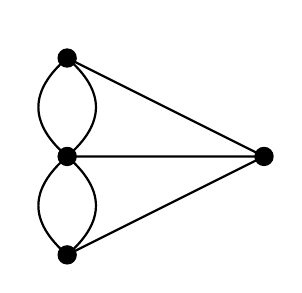
\begin{tikzpicture}[yscale=.5, scale=1.25]
 \draw[thick] (-1,-2) \v to [out=120, in=240] (-1,0) \v to [out=120, in=240] (-1,2) \v to [out=300, in=60] (-1,0) to [out=300, in=60] (-1,-2);
  \draw[thick] (1,0) \v -- (-1,2) (-1,0) -- (1,0) -- (-1,-2);
  \end{tikzpicture}
\end{center}

\begin{solution}
Try to draw an Euler circuit and see where you get stuck.  Connect this vertex to another that still has unused edges incident to it.  You can do this once to get an graph that has an Euler path, but to get an Euler circuit you will need to add two edges.
\end{solution}

\question Below is {\em part} of a graph.  Even though you can only see some of the vertices, can you deduce whether the graph will have an Euler path or circuit?

\begin{center}
 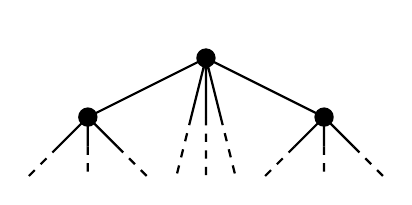
\begin{tikzpicture}[scale=.75]
  \draw[thick] (-2,0) \v -- (0,1) \v -- (2,0) \v;
  \draw[thick] (-2,0) -- (-2.5, -.5) (-2,0) -- (-2, -.5) (-2,0) -- (-1.5,-.5);
  \draw[thick, dashed] (-2.5, -.5) -- (-3, -1) (-2,-.5) -- (-2,-1) (-1.5,-.5) -- (-1,-1);
    \draw[thick] (2,0) -- (2.5, -.5) (2,0) -- (2, -.5) (2,0) -- (1.5,-.5);
  \draw[thick, dashed] (2.5, -.5) -- (3, -1) (2,-.5) -- (2,-1) (1.5,-.5) -- (1,-1);
    \draw[thick] (0,1) -- (-.25, 0) (0,1) -- (0, 0) (0,1) -- (.25,0);
  \draw[thick, dashed] (-.25, 0) -- (-.5, -1) (0,0) -- (0,-1) (.25,0) -- (.5,-1);
 \end{tikzpicture}

\end{center}

\begin{solution}
The graph will not have an Euler path or circuit.  To use up all the edges on the outer vertices, you will need to start at one and stop at the other.  But then you will have only used an even number of the edges at the middle vertex (an equal number ``in'' and ``out'').
\end{solution}


\newpage

%\uplevel{The {\em degree} of a vertex is the number edges connected to it.  Is there a connection between the degrees of vertices and the existence of Euler paths and circuits?  Let's find out.}

%\question List the degrees of each vertex of the graphs below.  Which graphs had Euler paths?  Which had Euler circuits?  What does this have to do with the vertex degrees?
%
%\begin{center}
% \begin{tikzpicture}
%  \draw[thick] (-1,0) \v -- (1,0)\v -- (1,2) \v -- (-1, 2) \v -- (-1,0) -- (1,2) (-1,2) -- (1,0) (0,1) \v;
%  \draw[thick] (-1,2) -- (0,3) \v -- (1,2);
%\end{tikzpicture}
%\hfill
% \begin{tikzpicture}
%  \draw[thick] (-1,0) \v -- (1,0)\v -- (1,2) \v -- (-1, 2) \v -- (-1,0) -- (1,2) (-1,2) -- (1,0) (0,1) \v;
%\end{tikzpicture}
%\hfill
% \begin{tikzpicture}
%  \draw[thick] (-1,0) \v -- (1,0)\v -- (1,2) \v -- (-1, 2) \v -- (-1,0) -- (1,2) (-1,2) -- (1,0) (0,1) \v;
%  \draw[thick] (-1,0) -- (-2,1) \v -- (-1,2) (1,2) -- (2,1) \v -- (1,0);
%\end{tikzpicture}
%\hfill
%\begin{tikzpicture}[yscale=.5]
% \draw[thick] (-1,-2) \v to [out=120, in=240] (-1,0) \v to [out=120, in=240] (-1,2) \v to [out=300, in=60] (-1,0) to [out=300, in=60] (-1,-2);
%  \draw[thick] (1,0) \v -- (-1,2) (-1,0) -- (1,0) -- (-1,-2);
%  \end{tikzpicture}
%
%\end{center}


%\vskip 3em
%\question Is it possible for a graph with a degree 1 vertex to have an Euler circuit?  If so, draw one.  If not explain why not.  What about an Euler path?
%\vfill
%
%\question What if every vertex of the graph has degree 2.  Is there an Euler path?  An Euler circuit?  Draw some graphs.
%\vfill
%
%\question Below is {\em part} of a graph.  Even though you can only see some of the vertices, can you deduce whether the graph will have an Euler path or circuit?
%
%\begin{center}
% \begin{tikzpicture}
%  \draw[thick] (-2,0) \v -- (0,1) \v -- (2,0) \v;
%  \draw[thick] (-2,0) -- (-2.5, -.5) (-2,0) -- (-2, -.5) (-2,0) -- (-1.5,-.5);
%  \draw[thick, dashed] (-2.5, -.5) -- (-3, -1) (-2,-.5) -- (-2,-1) (-1.5,-.5) -- (-1,-1);
%    \draw[thick] (2,0) -- (2.5, -.5) (2,0) -- (2, -.5) (2,0) -- (1.5,-.5);
%  \draw[thick, dashed] (2.5, -.5) -- (3, -1) (2,-.5) -- (2,-1) (1.5,-.5) -- (1,-1);
%    \draw[thick] (0,1) -- (-.25, 0) (0,1) -- (0, 0) (0,1) -- (.25,0);
%  \draw[thick, dashed] (-.25, 0) -- (-.5, -1) (0,0) -- (0,-1) (.25,0) -- (.5,-1);
% \end{tikzpicture}
%
%\end{center}


\question Edward A. Mouse has just finished his brand new house.  The floor plan is shown below:

\begin{center}
  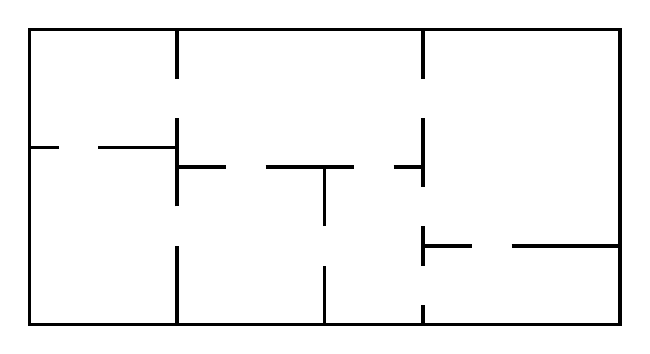
\begin{tikzpicture}[scale=1.25]
    \draw[very thick] (-3,0) rectangle (3,3);
    \draw[very thick] (-3,1.8) --(-2.7,1.8) (-2.3,1.8) -- (-1.5, 1.8) (-1.5, 1.6) -- (-1,1.6) (-.6, 1.6) -- (.3,1.6) (.7,1.6) -- (1, 1.6) (1, .8) -- (1.5, .8) (1.9,.8) -- (3,.8);
    \draw[very thick] (-1.5,0) -- (-1.5, .8) (-1.5, 1.2) -- (-1.5,2.1) (-1.5,2.5) -- (-1.5,3);
    \draw[very thick] (0,0) -- (0,.6) (0,1) -- (0,1.6);
    \draw[very thick] (1,0) -- (1,.2) (1,.6) -- (1,1) (1,1.4) -- (1,2.1) (1,2.5) -- (1,3);
  \end{tikzpicture}
\end{center}


Edward wants to give a tour of his new pad to a lady-mouse-friend.  Is it possible for them to walk through every doorway exactly once?  If so, in which rooms must they begin and end the tour? Explain.
 % \begin{solution}
 %   Yes, he must start in the top right room and end in the bottom middle room, or vice versa.  This is because those are the two rooms with an odd number of doors.
 %
 %   In graph theory terms, if we place a vertex in each room and connect vertices if there is a door between their rooms, we are asking whether the graph has an Euler path.  The number of doors is the degree of the vertex, and a graph has an Euler path if and only if there are two or fewer vertices with odd degree.  In that case, the path must start at one of those odd degree vertices and end at the other.
 % \end{solution}


\end{questions}
\end{document}
